\section{temp}
\subsection{Visitor Pattern}
\begin{frame}{Traversing the Tree}
\framesubtitle{Visitor Pattern}
	\begin{itemize}
        \item ANTLR visitor pattern
        \item Our own Visitor Pattern
    \end{itemize}
    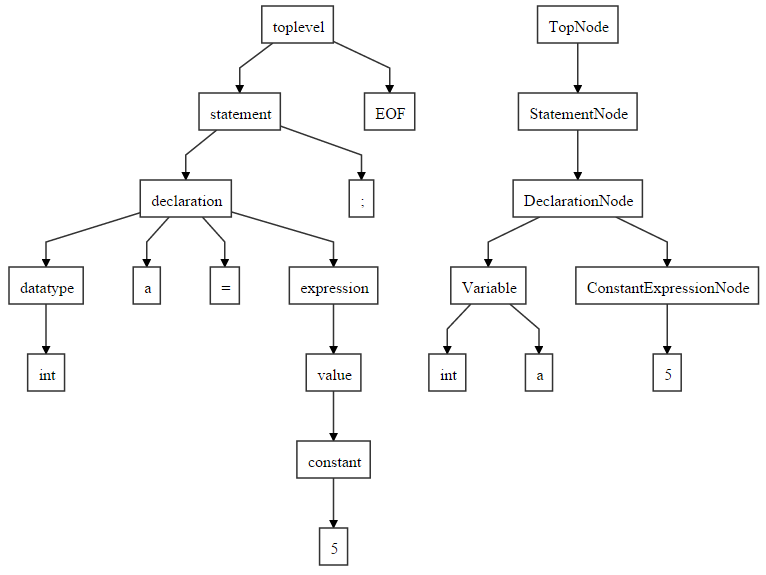
\includegraphics[width=1\textwidth,height=0.7\textheight,keepaspectratio, , clip]{images/P4/AST.PNG}

\end{frame}

\begin{frame}[fragile]{Contextual Analysis}
\framesubtitle{Module call}



\begin{lstlisting}[caption=The visit method for visiting a DeclarationNode in the code generator. ,frame=tlrb,label={lst:DeclarationNodeCodeGen}]
@Override
public String VisitDeclarationNode(DeclarationNode node) {
    String expr = "";
    String complexType = "";
    if (node.getExpression() != null){
        resultVarStack.push(node.getVariable());
        expr = visit(node.getExpression());
        resultVarStack.pop();
    }

    if (node.getVariable().isComplex()) {
        ...
    }
    if (expr.indexOf("sclManageArgsLaunchKernel
    	(hardware, software, global_size, local_size") >= 0){
        ...
    }

    return complexType.length() > 0 ? complexType + expr :
    (node.getVariable().toCcode() + " = " + expr + ";");
}
\end{lstlisting}
\end{frame}